\chapter{PyTorch编程}
\label{cp:pytorch}

\section{简介}

\textbf{PyTorch是一个以灵活性和易用性著称的深度学习框架},它的设计目标是\textbf{支持动态计算图}。与静态计算图的框架(如TensorFlow的早期版本)不同,\textit{PyTorch的计算图是在每次前向传播时动态生成的},故而它在\textit{进行调试和处理复杂模型时具有更大的灵活性}。\textbf{PyTorch的基本构件是张量(tensor)},它是一个多维数组,类似于NumPy的数组,但不同之处在于PyTorch的张量\textbf{可以使用GPU进行加速计算}。本次实验,我们在Windows系统上配备了NVIDIA显卡的情况下,就\textbf{可以通过CUDA加速神经网络的训练过程}。

\section{安装与配置}

需要首先\textbf{安装支持CUDA的PyTorch版本}。首先应该确定自己的显卡型号,可以使用命令\texttt{nvidia-smi}查看,其中包含了\textbf{CUDA版本},然后前往\href{https://pytorch.org/get-started/locally/}{PyTorch官网}查看支持自己的版本,找到对应的安装命令。例如,对于CUDA 12.4,可以使用如下命令安装:

\begin{minted}{bash}
pip3 install torch torchvision torchaudio --index-url https://download.pytorch.org/whl/cu124
\end{minted}

若未安装过\textit{CUDA},还需要前往\href{https://developer.nvidia.com/cuda-downloads}{NVIDIA官网}下载并安装。\\

安装过程会比较耗时,安装完成后,可以检查是否安装成功:

\begin{minted}{bash}
python3 -c "import torch; print(torch.__version__)"
\end{minted}

成功安装的输出如图\ref{fig:pytorch-version}所示。

\begin{figure}[htbp]
    \centering
    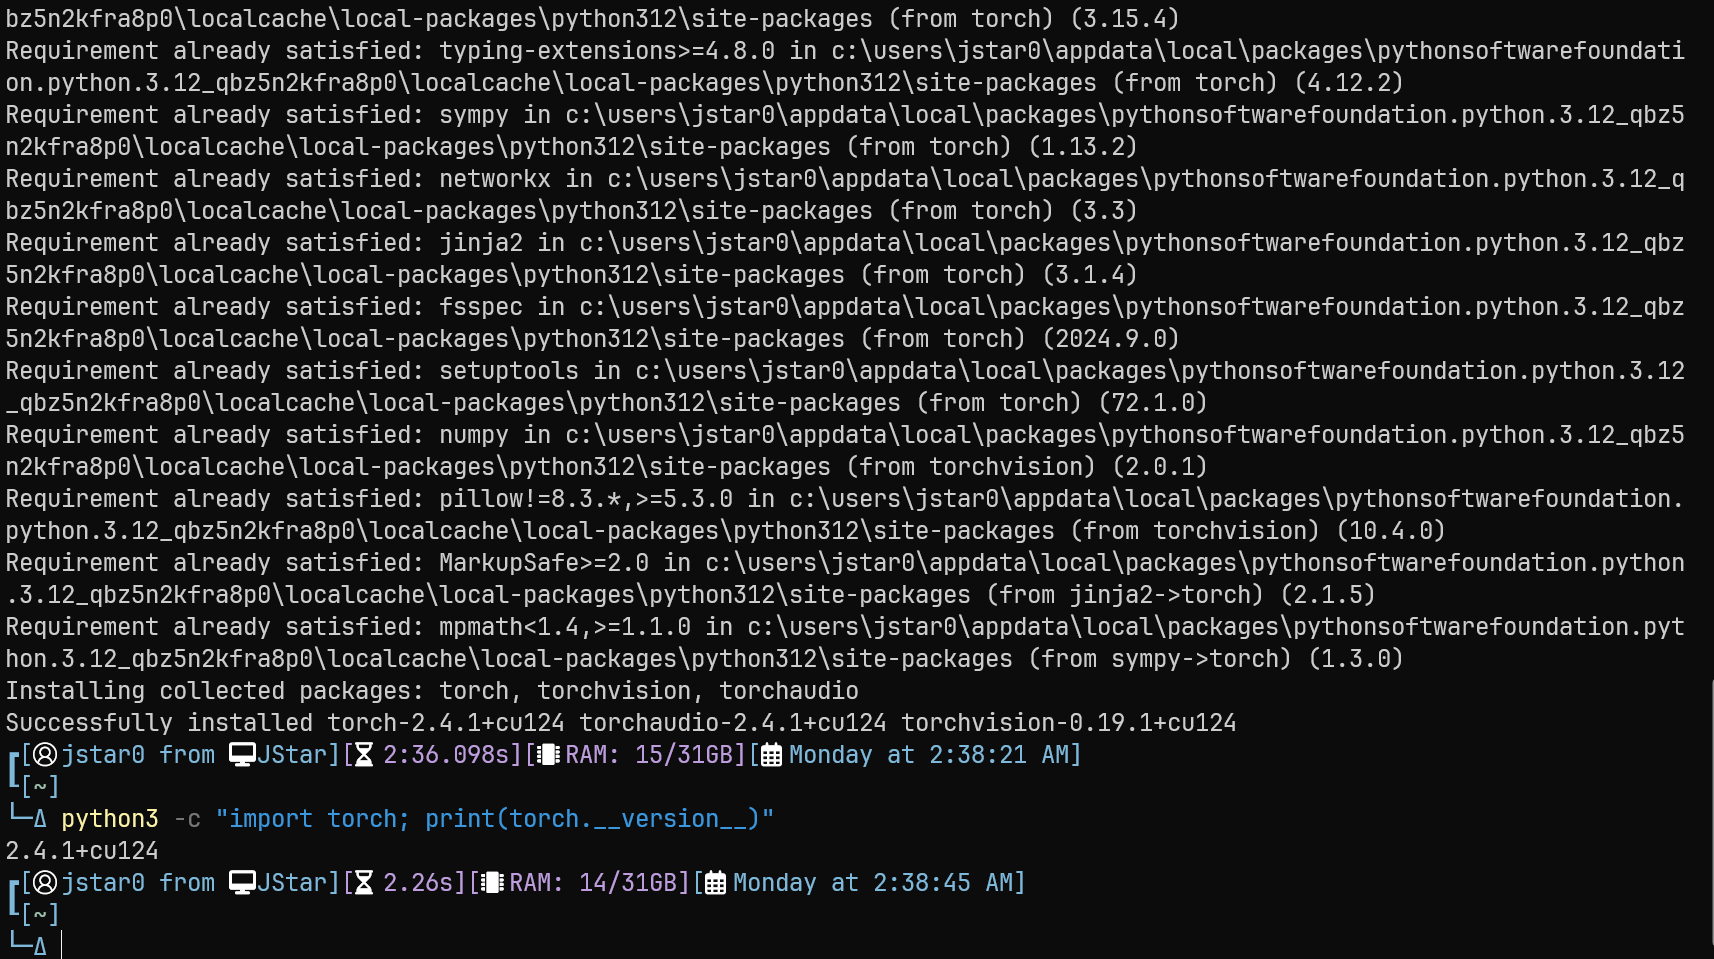
\includegraphics[width=0.9\textwidth]{Figures/installtorch.png}
    \caption{PyTorch安装成功检测}
    \label{fig:pytorch-version}
\end{figure}

\section{基本张量并用GPU加速}

我们可以创建一个2行3列的随机张量,如果\textit{torch.cuda.is\_available() == True}函数满足(判断是否有可用的GPU),将张量移动到GPU上,加速随后的计算操作。示例如代码\ref{listing:pytorch-tensor}所示。

既然安装成功,我们就可以开始编写PyTorch程序了。我们首先创建一个随机初始化的张量,然后将其移动到GPU上,请见代码\ref{listing:pytorch-tensor}。

\begin{longlisting}
    \begin{minted}{python}
import torch

# 创建一个随机初始化的张量
tensor = torch.rand(2, 3)

# 将张量移动到GPU上
if torch.cuda.is_available():
    tensor = tensor.to('cuda')
    print("GPU加速成功!")
    
print(tensor)
    \end{minted}
    \caption{PyTorch基本张量与GPU加速}
    \label{listing:pytorch-tensor}
\end{longlisting}

一切顺利,我们就可以看到如图\ref{fig:pytorch-tensor}所示的输出。

\begin{figure}[htbp]
    \centering
    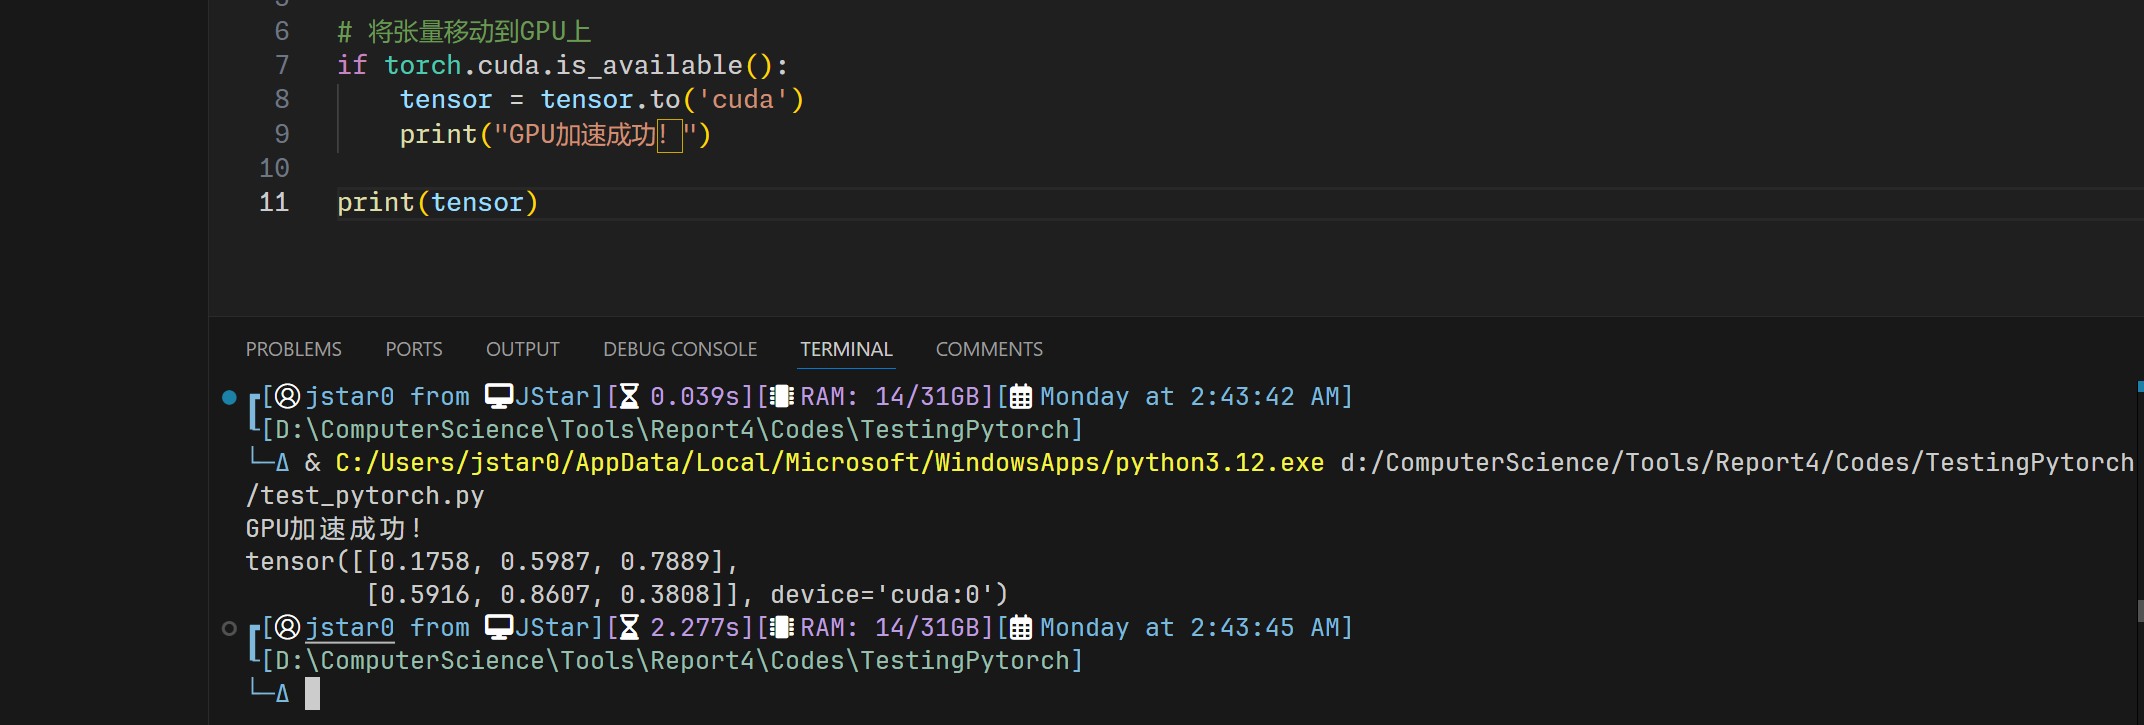
\includegraphics[width=\textwidth]{Figures/cudaOK.png}
    \caption{PyTorch基本张量与GPU加速成功}
    \label{fig:pytorch-tensor}
\end{figure}

\section{构建一个简单的神经网络}

这部分内容过于专业与复杂,我们只得借鉴他人的成功实践。\\

例子中,我们\textbf{定义了一个包含三层的简单全连接神经网络},\textit{输入维度为10,输出维度为1}。\texttt{forward}函数定义了\textit{前向传播的过程},使用\texttt{ReLU}激活函数来\textit{引入非线性}。模型初始化后,我们同样\textit{通过判断是否有可用的GPU,将整个网络结构移动到GPU上}。这种情况下,网络的所有计算操作都将在GPU上完成,极大地提高了计算速度。示例如代码\ref{listing:pytorch-nn}所示。

\begin{longlisting}
    \begin{minted}{python}
import torch
import torch.nn as nn
import torch.optim as optim

# 定义一个简单的神经网络
class SimpleNet(nn.Module):
    def __init__(self):
        super(SimpleNet, self).__init__()
        self.fc1 = nn.Linear(10, 50)
        self.fc2 = nn.Linear(50, 20)
        self.fc3 = nn.Linear(20, 1)

    def forward(self, x):
        x = torch.relu(self.fc1(x))
        x = torch.relu(self.fc2(x))
        x = self.fc3(x)
        return x

# 初始化网络并将其移动到GPU
net = SimpleNet()
if torch.cuda.is_available():
    net = net.to('cuda')

# 打印网络结构
print(net)
    \end{minted}
    \caption{PyTorch构建简单神经网络}
    \label{listing:pytorch-nn}
\end{longlisting}

如果一切顺利,则有如图\ref{fig:pytorch-nn}所示的输出。

\begin{figure}[htbp]
    \centering
    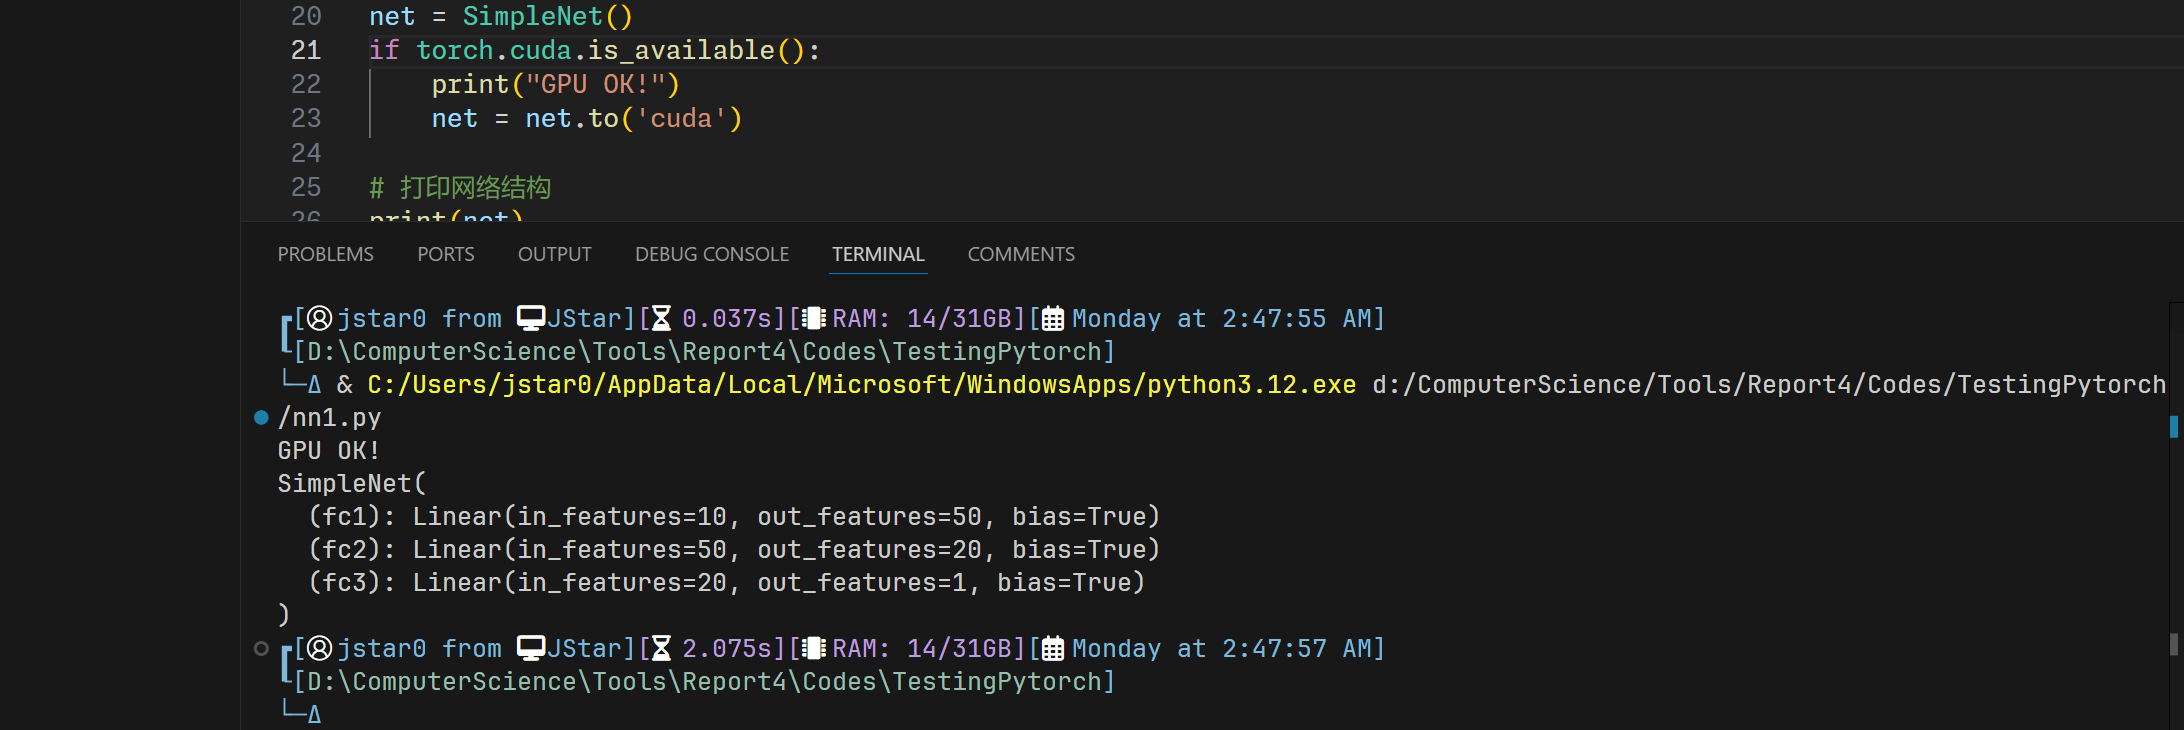
\includegraphics[width=\textwidth]{Figures/nn1.png}
    \caption{PyTorch构建简单神经网络成功}
    \label{fig:pytorch-nn}
\end{figure}

最后,我们\textbf{尝试如何对神经网络送入数据}。PyTorch提供了强大的数据处理模块\texttt{torch.utils.data},用于\textit{加载、处理数据,并将数据批量送入神经网络进行训练}。以下示例展示了如何使用PyTorch的\textit{DataLoader}加载数据,并将其送入网络进行前向传播,见代码\ref{listing:pytorch-dataloader}。

\begin{longlisting}
    \begin{minted}{python}
import torch
import torch.nn as nn
from torch.utils.data import DataLoader, TensorDataset

# 定义一个最简单的神经网络
class SimpleNet(nn.Module):
    def __init__(self):
        super(SimpleNet, self).__init__()
        # 线性层的输入大小为10,输出大小为1
        self.fc = nn.Linear(10, 1)

    def forward(self, x):
        # 前向传播:直接输出线性层的结果
        return self.fc(x)

# 创建网络实例
net = SimpleNet()

if torch.cuda.is_available():
    net = net.to('cuda')

# 创建一些随机数据
inputs = torch.randn(100, 10)  # 100个样本,每个样本10个特征
targets = torch.randn(100, 1)  # 对应的目标值

# 创建数据集和数据加载器
dataset = TensorDataset(inputs, targets)
dataloader = DataLoader(dataset, batch_size=16, shuffle=True)

# 在训练循环中加载数据并进行前向传播
for batch_inputs, batch_targets in dataloader:
    if torch.cuda.is_available():
        batch_inputs, batch_targets = batch_inputs.to('cuda'), batch_targets.to('cuda')
    
    outputs = net(batch_inputs)
    print(outputs)
    \end{minted}
    \caption{PyTorch使用DataLoader加载数据}
    \label{listing:pytorch-dataloader}
\end{longlisting}

我在示例代码所做的工作是,\textbf{创建一个最简单的神经网络SimpleNet},然后将其实例化为\texttt{net},并移动到GPU上。其余部分的训练参考了网上的代码。如果一切顺利,我们就可以看到如图\ref{fig:pytorch-dataloader}所示的输出。

\begin{figure}[htbp]
    \centering
    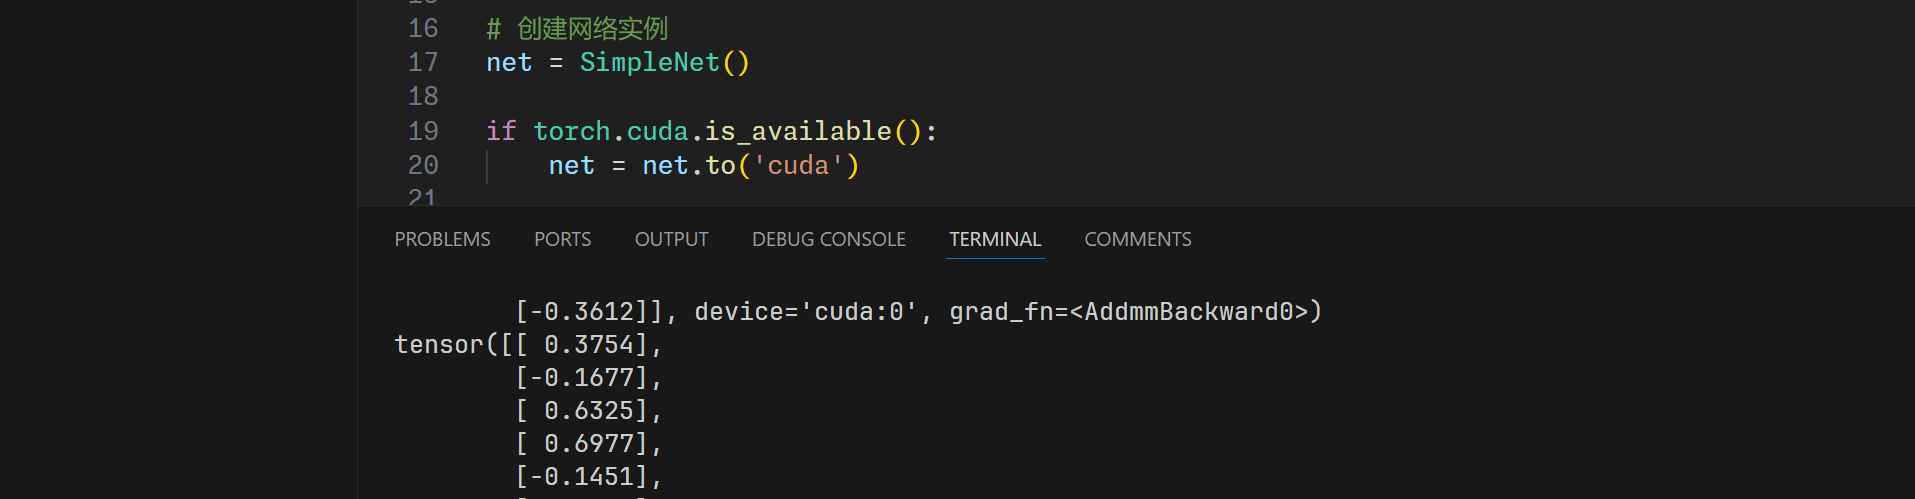
\includegraphics[width=\textwidth]{Figures/dataloader.png}
    \caption{PyTorch使用DataLoader加载数据成功}
    \label{fig:pytorch-dataloader}
\end{figure}